\documentclass[12pt,a4paper,twoside,titlepage]{article}
\usepackage[utf8]{inputenc}
\usepackage[english]{babel}
\usepackage{utopia}
\usepackage[margin=1in]{geometry}
\usepackage[parfill]{parskip}
\usepackage{makeidx}
\usepackage{graphicx}
\usepackage[onehalfspacing]{setspace}
\usepackage{fancyhdr}
%\usepackage{lastpage}
\usepackage{hyperref}
\renewcommand{\sffamily}{phv}

\newcommand{\titleText}{DHCP Aufgabe Dokumentation}
\newcommand{\authorText}{Patrick Günthard}
\newcommand{\dateText}{\today}

\title{\textbf{M123}\\\titleText}
\author{\authorText}
\date{\dateText}

\pagestyle{fancy}
\fancyhf{}

\fancyhead[EL]{\textbf{M123} \titleText}
\fancyhead[OR]{\authorText}
\cfoot{\thepage}% \space von \pageref{LastPage}}

\begin{document}
	\maketitle
	\tableofcontents

        \section{Software Basis}

        \begin{tabular}{|l|p{7cm}|}
          \hline
          \textbf{Virtualisierungs-Software} & Oracle VirtualBox 5\\\hline
          \textbf{Server OS} & Debian GNU/Linux 8 Jessie (Im Text einfachheitshalber \textit{Debian-Server} oder \textit{Debian-System} genannt.)\\\hline
          \textbf{Client OS} & Windows Server 2012 R2 (Im Text einfachheitshalber \textit{Windows-Client} oder \textit{Windows-System} genannt.) \\\hline
          \textbf{DHCP Server} & isc-dhcp-server \\\hline
        \end{tabular}

        \section{Aufgabenstellung}

        Die grundlegende Aufgabe bestand darin, auf einer Linux-VM einen DHCP Server zu installieren und diesen dann mit einem Windows-Client (ebenfalls auf einer VM) zu testen.

        \paragraph{Aufgaben}
        \begin{enumerate}
        \item Installation der VM
          \begin{itemize}
          \item Debian GNU/Linux 8
          \item Microsoft Windows Server 2012
          \end{itemize}
        \item Installation des DHCP Servers
        \item Konfiguration des Netzwerks
        \item Konfiguration des DHCP Servers
        \item starten des DHCP Servers
        \item Netzwerk Konfiguration auf dem Windows-Client
        \item Testen auf dem Windows-Client
        \end{enumerate}

        \section{Vorgehen}

        \subsection{Hürden}

        Es gab verschiedene Hürden beim aufsetzten des DHCP-Servers. Zu begin war nicht klar, welches package installiert werden sollte, da im Debian-Repository mehrere Implementierungen vorhanden sind. Ich entschied mich dann für den \textit{isc-dhcp-server} welcher weit verbreitet ist.
        
        Bei der Konfiguration des DHCP Servers gab es mehrere Probleme. Die im Aufgabenblatt beschriebenen Files existierten für das installierte Packet nicht sodass ich im Internet nach Lösungen suchen musste. Nach einiger Zeit ist es mir auch gelungen den Server richtig zu konfigurieren und ohne Fehler zu starten.
        \subsection{Lösungen}
        
        
        \begin{tabular}{lp{10cm}}
        	Konfiguration der VirtualBox & Bei der virtuellen Maschine des Servers muss eine zweite virtuelle Netzwerkkarte hinzugefügt werden. Es wird die Einstellung \textit{Internes Netzwerk} verwendet (Figure \ref{vboxconfig})\\
            DHCP Server & Das Packet \textit{isc-dhcp-server} eignet sich sehr gut für diese Aufgabe \\
            IP Konfiguration & Für eine korrekte verwendung muss die IP Adresse des Servers manuell gesetzt werden. Auf Unix-artigen Systemen wird dafür \textit{ifconfig} verwendet: \texttt{sudo ifconfig eth1 172.20.1.1 netmask 255.255.255.192}\\
            DHCP Konfiguration & Für die Konfiguration des DHCP Servers müssen 2 Dateien im \texttt{/etc/} modifiziert werden. Zum einen muss \texttt{/etc/default/isc-dhcp-server} modifiziert werden. Hier muss angegeben werden, auf welchem Netzwerk Interface der DHCP Server laufen wird. Wie schon im Beispiel der IP-Konfiguration wird hier das Interface \texttt{eth1} angegeben (Figure \ref{iscdhcpserver}). Auch muss die Datei \texttt{/etc/dhcp/dhcpd.conf} modifiziert werden (Figure \ref{dhcpdconf}). Hier muss die korrekte IP-Range definiert werden.\\
	        DHCP Server starten & Der DHCP Server wird mit dem Befehl \texttt{sudo /etc/init.d/isc-dhcp-server start} gestartet.\\
	        Windows-Client Konfigurieren & Standardmässig muss man den Windows-Client nicht konfigurieren, da dieser normalerweise das abrufen einer IP-Adresse über ein DHCP Server bereits aktiviert hat. Ist dies nicht der Fall, kann man dies über das Control-Panel nachholen: Control-Panel / Network and Internet / Network and Sharing Center / \textit{Your active Connection} / Properties / IPv4/v6 / Properties / Optain an IP Address automatically.
        \end{tabular}
        
        

		\begin{figure}
			\hrulefill\\
			\texttt{INTERFACES="eth1"}
			\caption{\label{iscdhcpserver} Konfiguration der Datei auf dem Pfad \texttt{/etc/default/isc-dhcp-server}}
			\hrulefill
		\end{figure}
		
		\begin{figure}
			\hrulefill\\
			\texttt{subnet 172.20.1.0 netmask 255.255.255.192 \{\\\hspace*{8pt} range 172.20.1.1 172.20.1.50;\\\}}\\
			\caption{\label{dhcpdconf} Konfiguration des IP-Ranges in \texttt{/etc/dhcp/dhcpd.conf}}
			\hrulefill
		\end{figure}


		\begin{figure}
			\hrulefill\\
			\center
			
			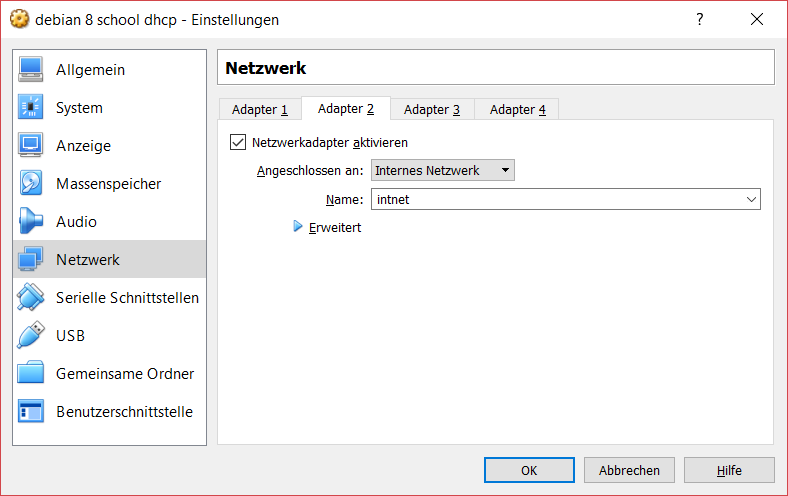
\includegraphics[width=8cm]{vbox_network_config}
			\caption{\label{vboxconfig} Netzwerk-Konfiguration der VirtualBox Maschine.}
			\hrulefill
		\end{figure}

		\section{Ergebnis \& Testprotokoll}
		
		\subsection{Ergebnis}
		
        \begin{figure}
          \hrulefill\\
          \center
          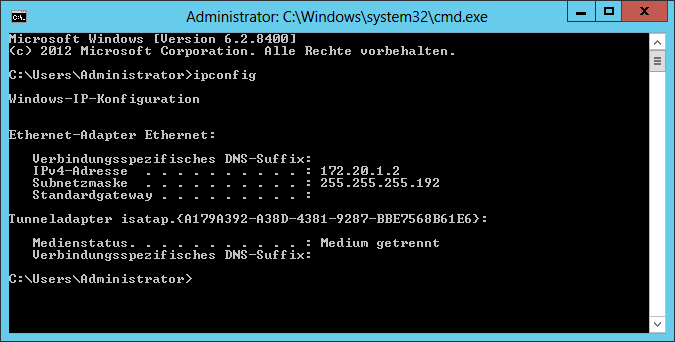
\includegraphics[width=8cm]{cmd_ipconfig_dynamic_ip}
          \caption{\label{dynip} Dynamisch zugewiesene IP auf Windows in \texttt{ipconfig}}
          \hrulefill
        \end{figure}

        \begin{figure}
	      \hrulefill\\
	      \center
          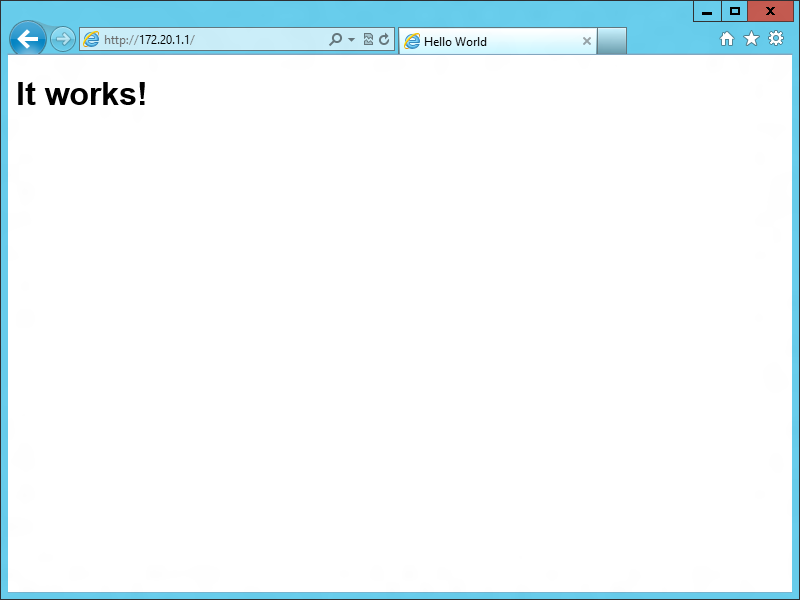
\includegraphics[width=8cm]{ie_web_example}
          \caption{\label{webserver} Erfolgreicher Zugriff vom Windows Client auf den Webserver auf dem Debian Server}
          \hrulefill
        \end{figure}
        
        Das Endergebnis war eine Debian 8 Maschine mit funktionierendem DHCP Server. Das richtige funktionieren des Servers wurde mit einem Windows-Client getestet welcher beim starten automatisch eine IP des im Server definierten Bereiches übernahm (Figure \ref{dynip}).

        Um zu testen ob auch eine Verbindung zwischen den beiden virtuellen Maschinen möglich ist, installierte ich auf dem Debian System ein Web-Server auf welchen ich auf dem Windows System erfolgreich zugreifen konnte (Figure \ref{webserver}).

        \subsection{Testprotokoll}


        \begin{tabular}{|l|l|p{7cm}|}
          \hline
          \textbf{Aufgabe} & \textbf{Status \ref{statusref}} & \textbf{Kommentar} \\\hline
          Virtual Box aufsetzen & E & - \\\hline
          OS installieren & E & \begin{itemize}
          \item Debian
          \item Windows
          \end{itemize} \\\hline
          Server konfigurieren & E & \begin{itemize}
          	\item IP Adresse festsetzen
          	\item DHCP Server konfigurieren
          	\item DHCP Server starten
          \end{itemize}\\\hline 
          Client OS konfigurieren & E & Automatische IP \\\hline
          System testen & E & \begin{itemize}
          	\item Wird der DHCP Server erfolgreich gestartet?
          	\item Bekommt der Windows-Client eine automatische IP?
          	\item Kann der Client mit dem Server kommunizieren?
          \end{itemize}\\\hline
        \end{tabular}

        \label{statusref}
        \textit{E} = erreicht, \textit{T} = teilweise erreicht, \textit{N} = nicht erreicht 
        
        \section{Reflexion}
        
        Die Aufgabe war für mich eine Herausforderung, wenn auch keine grosse. Da ich schon einige Erfahrungen im Betrieb von Applikationen dieser Art auf GNU/Linux Systeme hatte, kam ich schnell voran bei der Konfiguration des DHCP Servers.
        
        
\end{document}
